\section{Example}
\label{sec:example}
In this section, we illustrate our \CodeIn{eXpress} approach with an example. \CodeIn{eXpress} takes as input two versions of a program and produces as output a regression test suite, with the objective of detecting behavioral differences (if any exist) between the two versions of program under test. Although \CodeIn{eXpress} analyzes assembly code of C\# programs, in this section, we illustrate the \CodeIn{eXpress} approach using program source code. 

    \begin{figure}[t]
    \centering
        %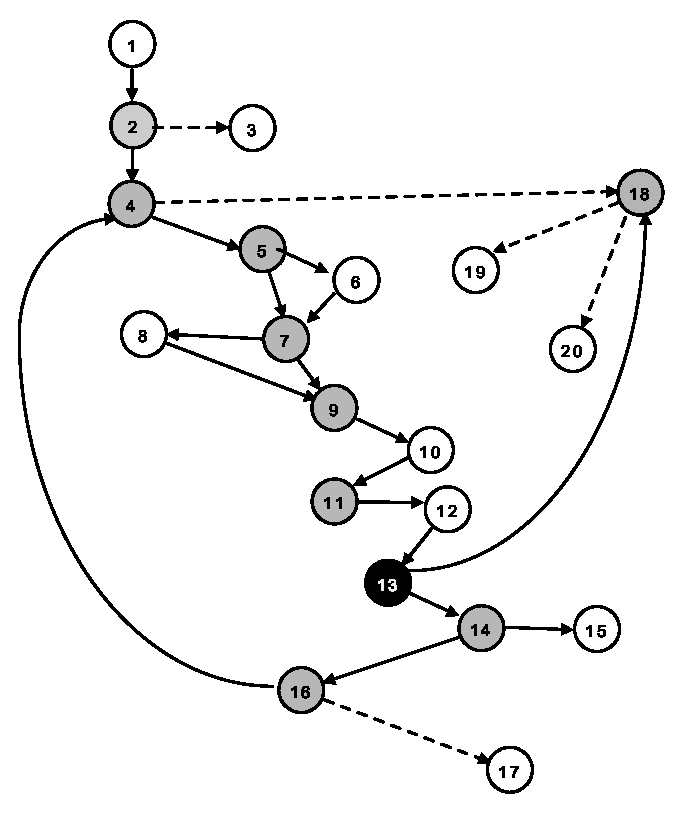
\includegraphics[width=6cm, keepaspectratio]{Figures/cfg3}
         \subfigure{\includegraphics[width=12.5cm, keepaspectratio]{Figures/example}}
         
    \vspace{-0.6cm}
    \caption{\scriptsize{An example program on the left side and the instrumented program on the right.}}
    \label{fig:example}
     \vspace{-0.7cm}
    \end{figure}
    
%\begin{figure}[t]
%
%%\begin{subfigure}
%\begin{CodeOut}
%\begin{alltt}
%
%  \hspace{0.25cm}\textbf{static public int} TestMe(\textbf{char[] }c, \textbf{int} n)\{
%1 \hspace{0.5cm} \textbf{int} state = 0;
%2 \hspace{0.5cm} \textbf{if}(c == \textbf{null} || c.Length == 0) 
%3 \hspace{0.75cm} \textbf{return -1;}   
%4 \hspace{0.5cm} \textbf{for}(\textbf{int} i=0; i< c.Length; i++)\{
%5 \hspace{1.0cm} \textbf{if}(c[i] == "[") state =1;
%6 \hspace{1.0cm} \textbf{else if}(state == 1 && c[i] == "\{") state =2;
%7 \hspace{1.0cm} \textbf{else if}(state == 2 &&  c[i] == "<") state =3;
%8 \hspace{1.0cm} \textbf{else if}(state == 3 && c[i] == "*")\{ 
%9 \hspace{1.25cm} state =4;
%10\hspace{1.25cm} \textbf{if}(c.Length==15) 
%11\hspace{1.5cm} state = state + n;//Added in new version
%	\hspace{1.0cm}   \}
%12\hspace{1.0cm} \textbf{if}(c[i]==' ') 
%13\hspace{1.25cm} \textbf{return};
%14\hspace{1.0cm} \textbf{if}(!(c[i] >= 'a' && c[i] <= 'z')\{
%15\hspace{1.25cm} state=-1; \textbf{return};
%  \hspace{1.0cm} \}
%  \hspace{.75cm} \}
%  \hspace{.50cm} \}
%16\hspace{.50cm} \textbf{if}(c[15] == '\}')
%17\hspace{.70cm} \textbf{return} state;
%18\hspace{.5cm} \textbf{return} -1;
%  \hspace{0.25cm}\}
%  
%\end{alltt}
%\end{CodeOut}
%\vspace{-0.9 cm}
%\caption{An example program}
%\label{fig:example}
%%\end{subfigure}
%
%\end{figure}
%
%\begin{figure}[t]
%\begin{CodeOut}
%\begin{alltt}
%
%  \hspace{0.25cm}\textbf{static public int} fOld(\textbf{int }state, 
%  \hspace{0.5cm}\textbf{int} length, \textbf{int} n)\{
%1 \hspace{0.5cm} \textbf{return} state;
%  \hspace{0.25cm}\}
%  
%  \hspace{0.25cm}\textbf{static public int} fNew(\textbf{int }state,
%  \hspace{0.5cm}\textbf{int} length, \textbf{int} n)\{
%1 \hspace{0.5cm} \textbf{if}(c.Length==15) state = state + n;
%2	\hspace{0.5cm} \textbf{return} state;
%  \hspace{0.25cm}\}
%  
%  \hspace{0.25cm}\textbf{static public int} TestMe(\textbf{char[] }c, \textbf{int} n)\{
%  \hspace{0.5cm} ...
%10\hspace{0.5cm} \textbf{int} stateCopy = state;
%11\hspace{0.5cm} state = fNew(state, c.Length, n);
%12\hspace{0.5cm} stateCopy = fOld(stateCopy, c.Length, n);
%13\hspace{0.5cm} if(state != stateCopy);   //Infection Condition
%  \hspace{0.5cm} ...
%  \hspace{0.25cm}\}
%\end{alltt}
%\end{CodeOut}
%\caption{Instrumentation to efficiently and effectively achieve I of the PIE model.}
%\vspace{-0.7 cm}
%\label{fig:example}
%\end{figure}


Consider the example in Figure~\ref{fig:example}. 
The left side of the figure shows a program \CodeIn{TestMe}. Lines 10 and 11 of the program are added in a new version.
\\ \textbf{Finding Irrelavant Branches.} 
%\CodeIn{eXpress} first compares the two program versions to find that Line 13 is added in the new version. \CodeIn{eXpress} then builds a Control-Flow Graph (CFG) of new version of  the program under test and marks the changed vertices in the graph.
The left side of Figure~\ref{fig:Tree} shows the CFG of the program in Figure~\ref{fig:example}. The labels of vertices in the CFG denote the corresponding line numbers in Figure~\ref{fig:example}. The black vertex denotes the newly added statements at Lines 10 and 11. The gray vertices denote the branching nodes (for the branching statements in the program), while the white vertices denote the other statements in the program. From the CFG, \CodeIn{eXpress} finds the following categories of branches.
%\\ \textbf{Difference Finder.} The Difference Finder component compares the original and the new versions of the program under test to find differences between each corresponding method of the two program versions. For the program in Figure~\ref{fig:example}, Difference Finder detects that the statements at Line 13 are added in the new version. 
%\\ \textbf{Graph Builder. }The Graph Builder component then builds a Control-Flow Graph (CFG) of the new version of  the program under test and marks the changed vertices in the graph. Figure~\ref{fig:CFG} shows the CFG of the program in Figure~\ref{fig:example}. The labels of vertices in the CFG denote the corresponding line numbers in Figure~\ref{fig:example}. The black vertex denotes the newly added statements at Line 13. The gray vertices denote the branching nodes (for the branching statements in the program), while the white vertices denote the other statements in the program.
%\\ \textbf{Graph Traverser.} The Graph Traverser component traverses the CFG to find each branch\footnote{\scriptsize{A branch is an outgoing edge of a branching node.}} $b$ in a program such that if $b$ is taken, the program execution cannot help in finding behavioral differences between the original and the new program versions. These branches are used by the Dynamic Test Generator component to efficiently find behavioral differences between the original and new program version.
%In particular, the Graph Traverser finds two categories of branches.
\begin{itemize}
\vspace{-1ex}
\item \textbf{Category $B_{E+I}$.} On traversing the CFG in Figure~\ref{fig:Tree}, \CodeIn{eXpress} detects that taking the branches $<$$2, 3$$>$\footnote{\scriptsize{$<$$x,y$$>$ represents a branch from source vertex $x$ to destination vertex $y$}}, $<$$4, 16$$>$, $<$$16, 17$$>$, $<$$16, 18$$>$, $<$$12, 13$$>$ and $<$$14, 15$$>$ (dotted edges in Figure~\ref{fig:Tree}), the program execution cannot reach any of the black vertices. Hence, the execution of these branches cannot help in executing the changed statements or infecting the program state. \\ 
\vspace{-1ex} 
\item \textbf{Category $B_{P}$.} In addition, \CodeIn{eXpress} finds out that 
among the source vertices of the six branches in Category $B_{I+E}$, there is no path from any of the 
black vertices to vertex 3. Hence, a state infection after the execution of the black vertex 
cannot propagate through the branch $<2,3>$.
\end{itemize}
\vspace{-0.2cm}
\textbf{Instrumentation for State Infection.}
A DSE-based test generation tool tries to execute all feasible branches in the program. However the execution of 
all branches is not sufficient for infecting the program state. For example, 
a test generation tool can 
cover all the branches of \CodeIn{}TestMe (left side of Figure~\ref{fig:example}) with $n=0$ (a default input used by some tools) but to infect the program state, the tool
need to generate a nonzero value of $n$.
To guide the test generation tool to effectively achieve state infection,
\CodeIn{eXpress} instruments the new program version.
In particular, \CodeIn{eXpress} invokes the changed regions\footnote{\scriptsize{A changed region (in a new or modified program version) is a minimal set of statements that contains all modified (in new or original program version), added (in new program version), or deleted (in original program version) statements in a method. The changed region for the new program version in \CodeIn{TestMe} on the left side of Figure~\ref{fig:example} is shown in rectangular box, while the changed region of the original program version is empty.}} 
from the two program versions (with same inputs) and 
compares the outputs of the two changed regions. 
\CodeIn{eXpress} inserts branches in the new program version that are executed only 
when the outputs of the executions of the changed regions differ, i.e., when program
state is infected after the execution of the changed regions.

The right side of Figure~\ref{fig:example} shows the instrumented version of \CodeIn{TestMe} on the left side of 
Figure~\ref{fig:example}. 
\CodeIn{eXpress} identifies $state$, $length$, and $n$ as the inputs to the two changed regions
and $state$ as the output to the two changed regions.
\CodeIn{eXpress} then extracts the
changed regions in the original and new program versions as separate methods 
(\CodeIn{fOld} and \CodeIn{fNew}, respectively).
The parameters of the two methods are same as the identified inputs, while the return values 
are same as the identified output.
%The method \CodeIn{fOld} shows the method extracted for the old program version,
%while the method \CodeIn{fNew} shows the method extracted for the new program version.
%Since the changed region in the old program version is empty, the method \CodeIn{fOld} just 
%returns $state$,
%while the method \CodeIn{fNew} contains Lines 10 and 11 (of \CodeIn{TestMe} on the 
%left side of Figure~\ref{fig:example}) and returns the resulting value of $state$.
\CodeIn{eXpress} replaces the changed region of the new version of
\CodeIn{TestMe} by the invocation of the methods \CodeIn{fOld} and \CodeIn{fNew} 
(Lines 11 and 12 on the right side of Figure~\ref{fig:example}). 
Note that the variable $stateOld$ passed to 
\CodeIn{fOld} is a copy of the variable $state$ passed to \CodeIn{fNew} (Line 10 on the right side of ~\ref{fig:example}) because 
$state$ may be updated by \CodeIn{fNew} since $state$ is also an output of the changed regions. 
\CodeIn{eXpress} then inserts an \CodeIn{if} statement (Line 13 on the right side of Figure~\ref{fig:example})
in the program comparing the outputs of the two methods.
Note that the outputs of the two methods are different if and only if the program state is infected.
A DSE-based test generation tool determines that it needs to generate inputs 
satisfying \CodeIn{c.Length == 15 AND state != state + n} to cover the true branch of the added \CodeIn{if} statement. 
Hence, the tool generates a nonzero value of $n$ to satisfy the constraint and infect the program state. 
\begin{figure}[t]
    \centering
        %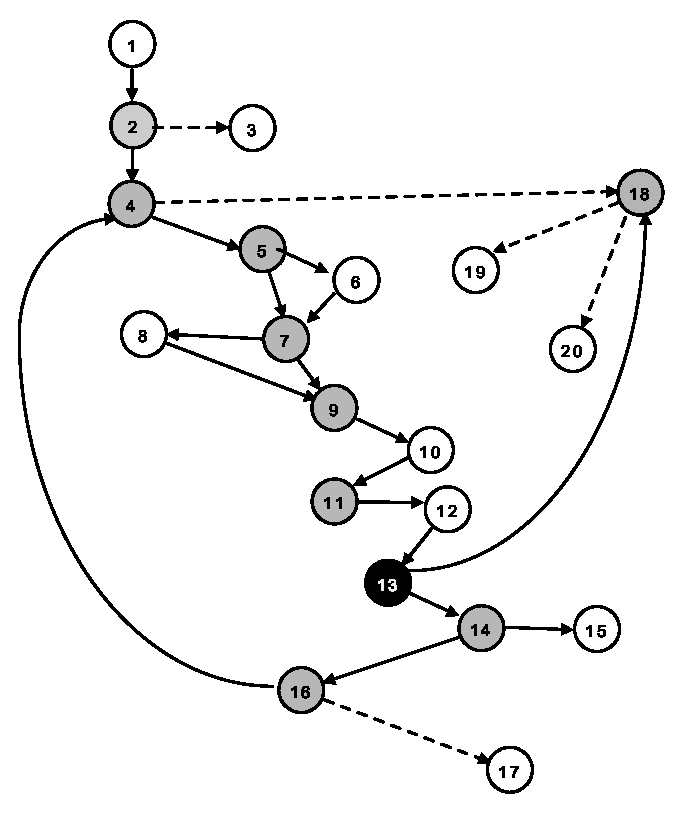
\includegraphics[width=6cm, keepaspectratio]{Figures/cfg3}
         \subfigure{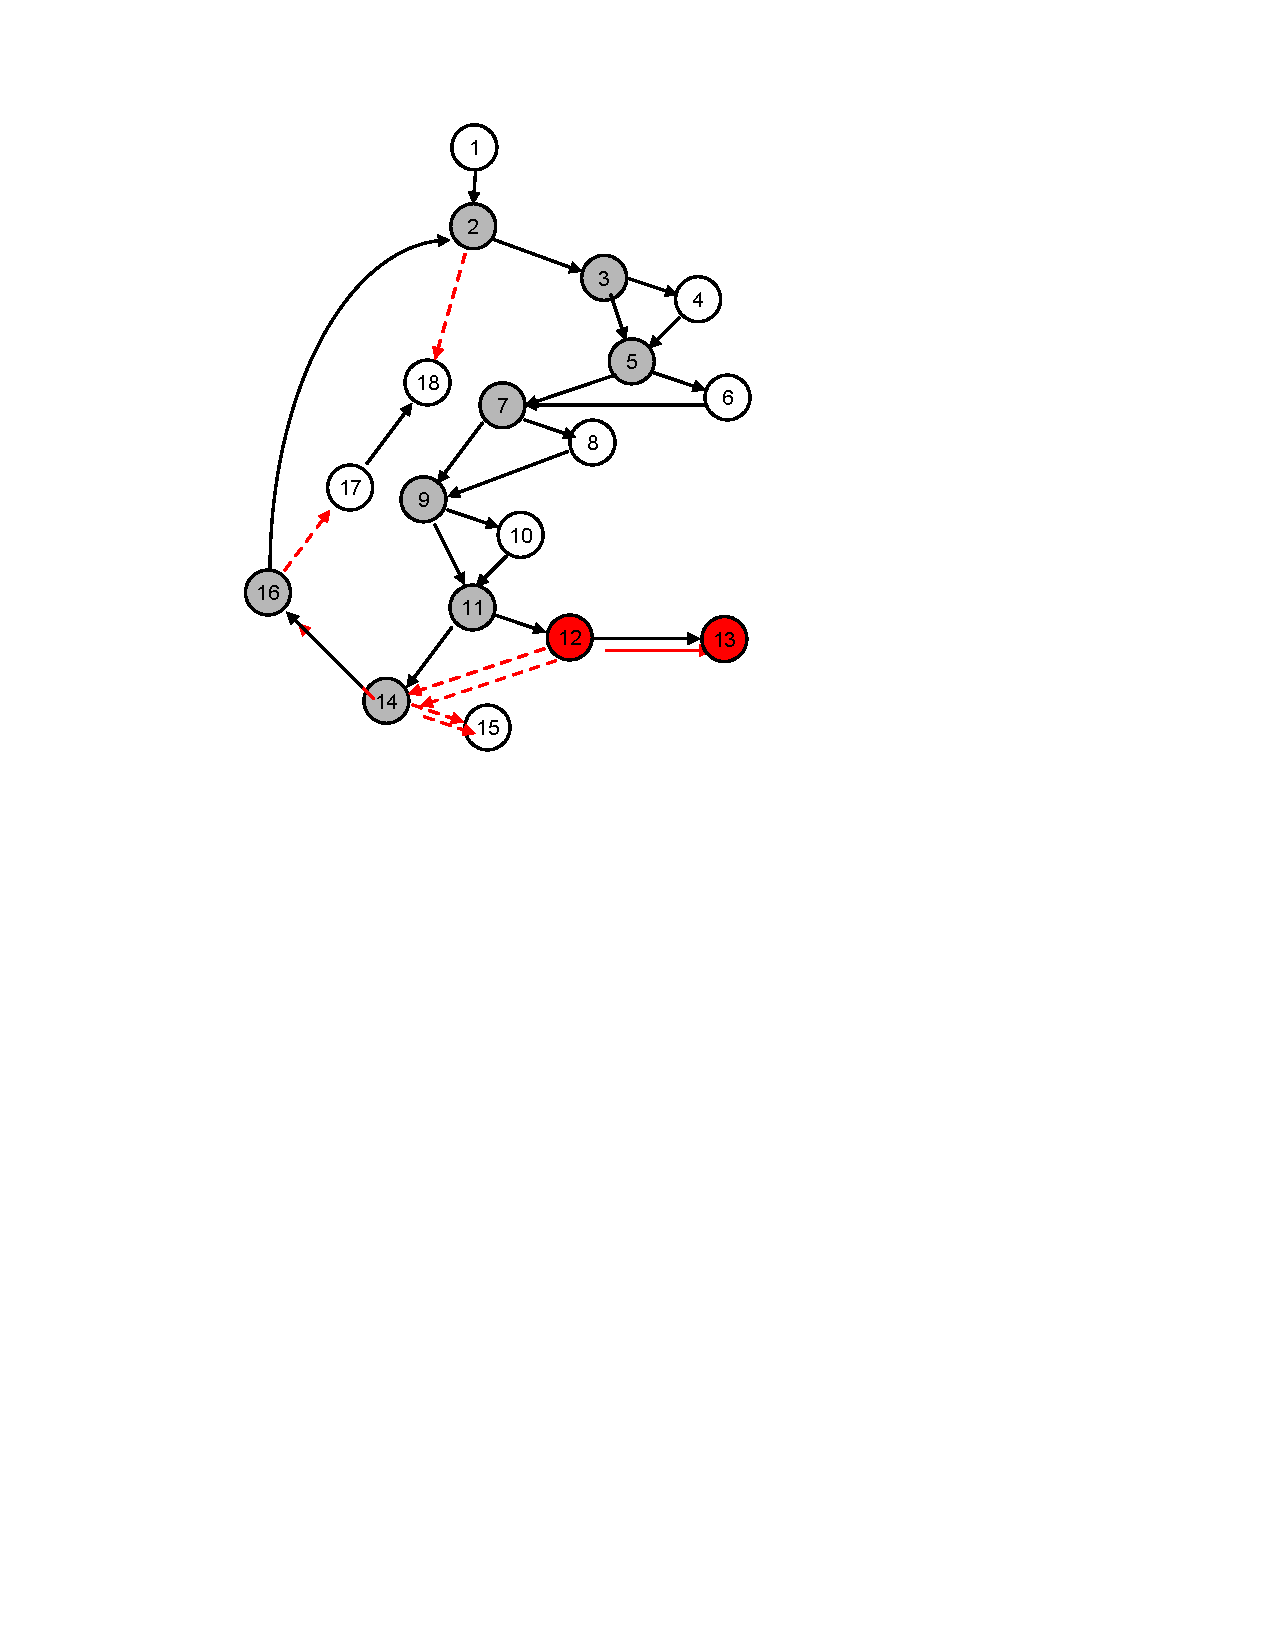
\includegraphics[width=4.5cm, keepaspectratio]{Figures/cfg}}
         \hspace{2cm}
         \subfigure{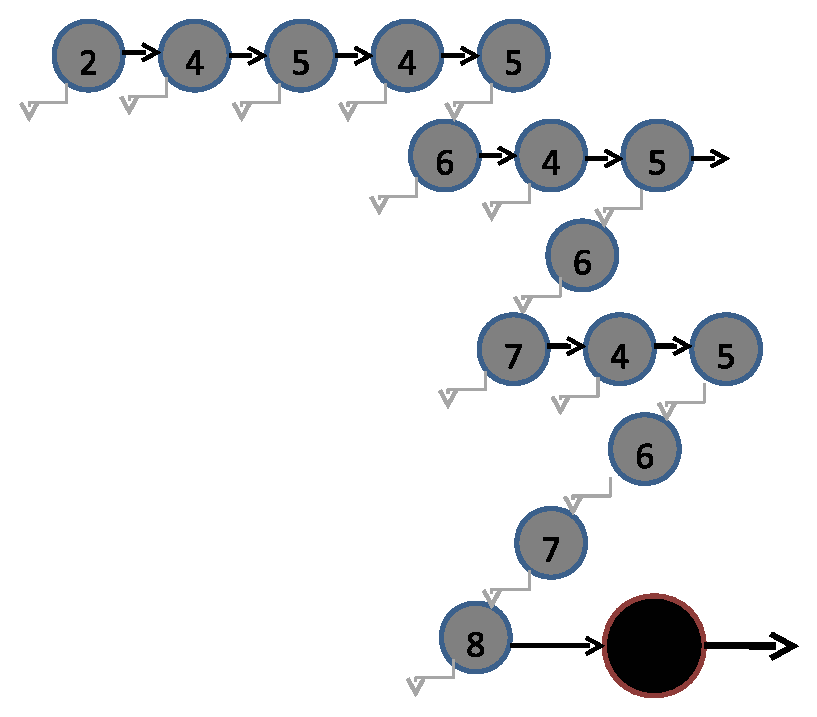
\includegraphics[width=4.5cm, keepaspectratio]{Figures/ExecutionTreeEPS}}
    \vspace{-0.4cm}
    \caption{\scriptsize{The left side of the figure shows the part of execution tree of the program for c = \{"[", "\{", "$<$", "*" \}, while the right side shows the Control-Flow Graph for the program in Figure~\ref{fig:example}.}}
    \vspace{-0.8cm}
    \label{fig:Tree}
    \end{figure}
%    \begin{figure}[t]
%    \centering
%        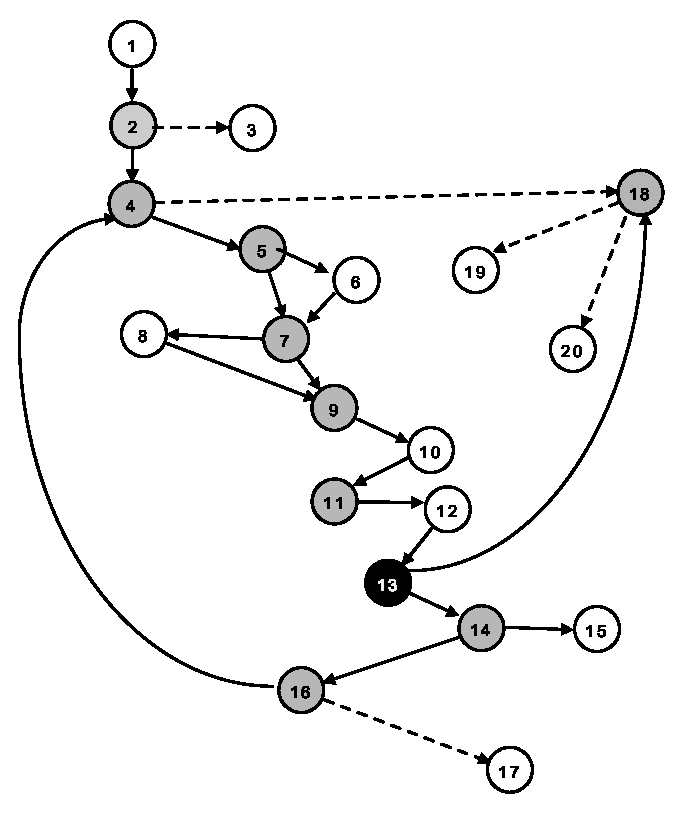
\includegraphics[width=4cm, keepaspectratio]{Figures/cfg3}
%        %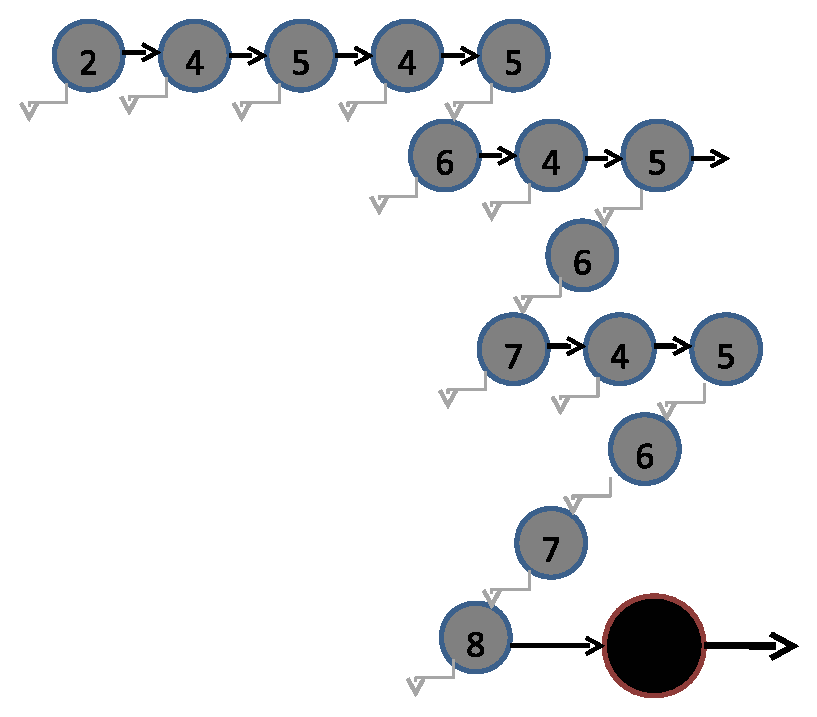
\includegraphics[width=4cm, keepaspectratio]{Figures/ExecutionTreeEPS}
%    \vspace{-0.2cm}
%    \caption{The Control-Flow Graph for the program in Figure~\ref{fig:example}}
%    \vspace{-0.5cm}
%    \label{fig:CFG}    
%	  \end{figure}
\Comment{
\\ \textbf{Instrumenter. }The Instrumenter component transforms the two versions of the
program code such that the transformed program code is
amenable to regression testing. In particular, the Instrumenter component
instruments both versions of the program under test so that program states can be compared (to determine state infection) after the execution of the added  statements at Lines 12 and 13.
}
\Comment{
	Figure~\ref{fig:Changed} shows the code of \CodeIn{testMe}'s new version after instrumentation. The \CodeIn{Instrumenter} component inserts a statement (Line 12 or 13 in Figure~\ref{fig:Changed}) just after any changed statement (Line 11 in Figure~\ref{fig:example}). The instrumented statement allows us to store the current value of \CodeIn{x} in a particular run (i.e., an explored path) of DSE. In particular, this statement results in an assertion \CodeIn{PexAssert.IsTrue ("uniqueName", x == currentX)}\footnote{\CodeIn{PexAssert} is an API class provided by Pex.} in the generated test, where \CodeIn{currentX} is the value of $x$ at Line 12 in the new version of the program. One such assertion is generated by Pex each time the statement is executed in the loop. Hence, if the loop containing the changed statement executes 20 times, 20 such assertions will be added to the test generated by Pex.
The generated test can be executed on the original version of \CodeIn{testMe} to compare program states at Line 12 after the execution of the changed statement with the ones captured in the execution of the new version. 			
\begin{figure}[t]
\begin{CodeOut}
\begin{alltt}
  \hspace{0.5cm}\textbf{public boolean} testMe(\textbf{int }x, \textbf{int[] } y)\{
  \hspace{1.0cm} ...
10\hspace{1.0cm} \textbf{if}(x == 110)\{	 
11\hspace{1.5cm} x = 2*j+1;
12\hspace{1.5cm} \textbf{PexStore.ValueForValidation}("uniqueName", x);
13\hspace{1.0cm} \} 
  \hspace{1.0cm} ...
  \}
\end{alltt}
\end{CodeOut}
\caption{Instrumented example program after instrumentation}
\label{fig:Changed}
\end{figure}
If there are multiple changed statements in the program, our approach first finds multiple regions each of which contains nearby changed statements in the program. We refer to each of such regions as a changed region in the rest of the paper. Our approach finds all the variables and fields that are identified as defined in a changed region and inserts statements (such as the statement at Line 12 of Figure \ref{fig:Changed}) to log the value of each defined variable or field in the changed region. If a defined variable is a non-primitive type, such a statement enables to compare the object graphs reachable from the logged values to compare program states. The \CodeIn{Dynamic Test Generator} component of \CodeIn{eXpress} then performs DSE on the instrumented new version of the program to generate regression tests. 
}
\Comment{
\CodeIn{eXpress} performs DSE on the instrumented new version of the program. After each run of DSE, \CodeIn{eXpress} executes the generated test on the instrumented original version (in the same way as instrumentation of the new version) to check whether the program state is infected after the execution of a changed region. The instrumentation enables us to perform only one instance of DSE on the new version instead of performing two instances of DSE: one on the original and the other on the new program version. Performing two instances of DSE can be technically challenging since we have to perform the two DSE instances in a controlled manner such that both versions are executed  with the same input and the execution trace is monitored for both the versions by a common exploration strategy to decide which branching node to flip next in the two versions. 

The Dynamic Test Generator component of \CodeIn{eXpress} uses Dynamic Symbolic Execution (DSE) to generate tests for the new version. DSE iteratively generates test inputs to cover various feasible paths in the program under test. In particular, DSE flips some branching node from a previous execution to generate a test input for covering a new path. The node to be flipped is decided by a search strategy (also called exploration starategy) such as depth-first search. Dynamic Test Generator implements a search strategy for Pex~\cite{Pex} to efficiently find behavioral differences between two versions of a program.
}
\\ \textbf{Test Generation. }To cover the changed statements at 
Lines 10 and 11 (in the left part of Figure~\ref{fig:example}) and infect the program state, 
 DSE needs at least 6 DSE runs (starting from an empty input array $c$). 
 However, the number of runs depends on the choice of branches that DSE flips in each run. 
 In each run, DSE has the choice of flipping 8 branches in the program. 
 For \CodeIn{TestMe}, Pex takes 441 DSE runs to cover the true branch of statement at Line 10. The number of runs can be much more if the number of branching statements in the program increases. To reduce the search space of DSE, \CodeIn{eXpress} prunes branches in category 
 $B_{E+I}$ until the black vertex is executed and the program state is infected after its execution.
 Once the program state is infected, \CodeIn{eXpress} prunes out the branches in category $B_{P}$ to efficiently propagate the state infection to an observable output.
\\ \textbf{Incremental Exploration.} \CodeIn{eXpress} can reuse an existing
test suite for the original version so that changed parts of the program can be explored
efficiently due to which test generation is likely to find behavior
differences earlier in path exploration. Assume that there is an existing test suite covering all the statements in the old version of the program in Figure~\ref{fig:example}. Suppose that the test suite has a test input $I$ = \{"[", "\{", "$<$", "*" \}. The input covers all the statements in the new version of \CodeIn{TestMe} except the newly added statement at Line 11. If we start the program exploration from a scratch (i.e., with default inputs), Pex takes 441 runs to cover the statement at Line 11. However, we can reuse the existing test suite for exploration to cover the new statement efficiently. Our approach executes the test suite to build an execution tree for the tests in the test suite. Our approach then starts program exploration using the dynamic execution tree built by executing the existing test suite instead of starting from an empty tree. Some branches in the tree may take many runs for Pex to discover if starting from an empty tree. Figure~\ref{fig:Tree} shows part of the execution tree for the input $I$. A gray edge in the tree indicates the false side of a branching node while a black (horizontal) edge indicates the true side. To generate an input for the next DSE runs, Pex flips a branching node $b$ in the tree whose other side has not yet been explored and generates an input so that program execution takes the unexplored branch of $b$. Pex chooses such branching node for flipping using various heuristics for covering changed regions of the program. It is likely that Pex chooses the branching node 13 (colored black), which on execution covers the \CodeIn{break} statement at Line 13. When starting the program exploration from scratch, Pex takes 420 runs before it reaches (discovers) the black branching node in Figure~\ref{fig:Tree}. Using our approach of seeding the tests from the existing test suite, Pex takes 39 runs to flip the branching node and cover the statement at Line 11.


\Comment{
\item \textbf{Branches not satisfying P}. Suppose the changed statement is executed, the program
state is infected after the execution of the changed statement, but the infection
does not propagate to an observable output.  We do
not explore the branches after the execution of the changed statement if these
branches do not lead to any other changed region.
}

\Comment{
For the example in Figure~\ref{fig:example}, our approach takes ** DSE runs to execute the changed statement, while the default strategy in Pex~\cite{Pex} takes ** DSE runs. To infect the program state, our approach takes ** DSE runs. The program state was propagated as soon as it was infected.
		}






\Comment{
\begin{figure}[t]
\begin{CodeOut}
\begin{alltt}
  [PexFactoryClass]
  \textbf{public class} FactoryClass\{
  \hspace{0.5cm}[PexFactoryMethod(typeof(\textbf{TestClassSynthesized}))]
  \hspace{0.5cm}\textbf{public static TestClassSynthesized} create(int a, 
  \hspace{1.5cm}int b, int c, int n)\{
  \hspace{1.0cm}\textbf{TestClassSynthesized} obj = 
  \hspace{1.5cm}\textbf{new} TestClassSynthesized(); 
  \hspace{1.0cm} \textbf{for}(int i=0; i< methodSeuenceLength; i++)\{
  \hspace{1.5cm} \textbf{switch}(n)
  \hspace{2.0cm} \textbf{case} 0: \textbf{obj}.A(a);\textbf{break};
  \hspace{2.0cm} \textbf{case} 1: \textbf{obj}.B(b);\textbf{break};
  \hspace{2.0cm} \textbf{case} 2: \textbf{obj}.C(c);\textbf{break};
  \hspace{2.0cm} \textbf{case} 3: \textbf{obj}.testMe();\textbf{break};
  \hspace{2.0cm} \textbf{default}: \textbf{break};
  \hspace{1.0cm}\}
  \hspace{1.5cm} \textbf{return} obj;
  \hspace{0.5cm}\}
  \}
\end{alltt}
\end{CodeOut}
\caption{Factory Class to generate an object of \CodeIn{TestClassSynthesized}}
\label{fig:factory}
\end{figure}
}




\Comment{
In this section, we illustrate our approach with the aid of an example. Our approach takes as input two versions of a class and produces as output a regression test suite. The test suite on execution detects behavioral differences between the two versions of class under test. Our approach is inspired by the PIE model~\cite{voas} of error propagation. According to the PIE model, a fault can be detected by a test suite if the fault is executed (E), the execution of the fault infects the state (I), and that the infected state propagates to the output (P). We have implemented our approach in Pex~\cite{Pex}, an automated structural testing tool based on for .NET developed at Microsoft Research. Pex uses Dynamic Symbolic Execution (DSE)~\cite{dart, cute} to explore various paths in the program and generate a unique test for each feasible path explored. To make the DSE efficiently in finding behavioral differences, our approach guides the DSE to avoid exploring irrelevant paths that cannot help in achieving E, I, or P of the PIE model.

\begin{figure}[t]
\begin{CodeOut}
\begin{alltt}
  \textbf{public} TestClass\{
  \hspace{0.5cm}\textbf{public boolean} testMe(\textbf{int }x, \textbf{int[] } y)\{
1 \hspace{1.0cm} \textbf{int} j=0, k=0;
2 \hspace{1.0cm} \textbf{if}(x==90)\{
3 \hspace{1.5cm} \textbf{for}(\textbf{int} i=0; i< y.Length; i++)\{
4 \hspace{2.0cm} \textbf{if}(y[i] == 15)
5 \hspace{2.5cm} x++;
6 \hspace{2.0cm} \textbf{else if}(y[i] == 25)
7 \hspace{2.5cm} \textbf{return} x;
8 \hspace{2.0cm} \textbf{if}(x >= 110 && x<= 150)
9 \hspace{2.5cm} j =1;
10\hspace{2.0cm} \textbf{else if}(x>150)
11\hspace{2.5cm} j =2;
12\hspace{2.0cm} \textbf{for}(i=200; i<= x; i++)
13\hspace{2.5cm} k++;
14\hspace{2.0cm} \textbf{if}(j > 0) // \textbf{if}(j >= 0)
15\hspace{2.5cm} x = j+2; //x = 2*j+1
16\hspace{2.0cm} \textbf{for}(int i=0; i< k+1; i++) 
17\hspace{2.5cm} x = x*k;
18\hspace{1.5cm} \}
19\hspace{1.0cm} \}
20\hspace{1.0cm} \textbf{return} x;
  \hspace{0.5cm}\}
  \hspace{0.5cm}...
  \hspace{0.5cm}A (\textbf{a})...
  \hspace{0.5cm}B (\textbf{b})...
  \hspace{0.5cm}C (\textbf{c})...
  \}  
\end{alltt}
\end{CodeOut}
\vspace{-0.15 in}
\caption{An Example Program}
\label{fig:example}
\end{figure}


Consider the example in Figure~\ref{fig:example}. Figure~\ref{fig:example} contains a class \CodeIn{TestClass}. The class \CodeIn{TestClass} contains a method \CodeIn{testMe} that has been changed in the new version. The class also contains 3 other methods \CodeIn{A}, \CodeIn{B}, and \CodeIn{C} that have not been changed in the new version. Suppose the statement at Line 15 of the method \CodeIn{testMe} has been modified to the one shown in the comment at Line 15. Our approach first constructs the control flow graph for the two versions and finds differences between the two control flow graphs. Our approach detects that Line 14 in the program has been changed. Instead of performing DSE separately for each version, our approach synthesizes a new class combining the two program versions as shown in Figure~\ref{fig:Changed}. As shown in Figure~\ref{fig:Changed}, our approach inserts an argument \CodeIn{isOriginalVersion} of type \CodeIn{boolean} in the method containing the changed statement. Our approach also inserts new branches at the location of changed statement(s). The \CodeIn{true} branch contains the original statement while the \CodeIn{false} branch contains the modified statement. The \CodeIn{true} branch is executed when \CodeIn{isOriginalVersion} is \CodeIn{true} and vice versa. The Line 15 in Figure~\ref{fig:example} has been changed to Lines 15-18 in Figure~\ref{fig:Changed}. The \CodeIn{true} branch of the \CodeIn{if} statement contains the original statement, while the false branch contains the statement in new version. The synthesized class \CodeIn{TestClassSynthesized} helps us in concurrently running the two versions without having to execute two instances of DSE on the two versions. After every run of DSE, we flip the \CodeIn{if(isOriginalVersion)} branch (if the branch is executed in that particular run) to check the program behavior in the new version. In the rest of this section we will refer to the program in Figure~\ref{fig:example}. Whenever we refer to comparison of program states after execution of the two versions under test, it means we flip the branch at Line 14 to execute the statement in the other version and compare the program states before and after flipping the branch. 

\begin{figure}[t]
\begin{CodeOut}
\begin{alltt}
  \textbf{public} TestClassSynthesized\{
  \hspace{0.5cm}\textbf{public boolean} testMe(\textbf{int }x, \textbf{int[] } y, 
  \hspace{3cm}\textbf{boolean} isOriginalVersion)\{
  \hspace{2.0cm} ...
14\hspace{2.0cm} \textbf{if}(j > 0)
15\hspace{2.5cm} \textbf{if}(isOriginalVersion)	 
16\hspace{3.0cm} x = j+2;
17\hspace{2.5cm} \textbf{else}
18\hspace{3.0cm} x = 2*j+1
  \hspace{2.0cm} ...
  \}
\end{alltt}
\end{CodeOut}
\vspace{-0.15 in}
\caption{Program synthesized for the example program}
\label{fig:Changed}
\end{figure}

Figure~\ref{fig:PUT} shows a Parameterized Unit Test for pex to generate tests for the method \CodeIn{testMe} in the class \CodeIn{TestClassSynthesized}. Figure~\ref{fig:factory} shows the factory method used for synthesizing an object for \CodeIn{TestClassSynthesized}. The factory method instantiates a new instance of the class \CodeIn{TestClassSynthesized}, generates a sequence of method calls containing all combinations \CodeIn{A}, \CodeIn{B}, \CodeIn{C}, and testMe. The length of the sequence is \CodeIn{methodSeuenceLength} which is set to total number of methods in the class \CodeIn{TestClassSynthesized} (4). 



\begin{figure}[t]
\begin{CodeOut}
\begin{alltt}
  [TestClass]
  \textbf{public class} PUTClass\{
  \hspace{0.5cm}[PexMethod]
  \hspace{0.5cm}\textbf{public boolean} testMePUT(\textbf{TestClassSynthesized} obj, int x, 
  \hspace{1.5cm}int[] y, boolean version)\{
 1\hspace{1.0cm}PexAssume.IsNotNull(obj);
 2\hspace{1.0cm}obj.testMe(x, y, version);
  \hspace{0.5cm}\}
  \}
\end{alltt}
\end{CodeOut}
\vspace{-0.15 in}
\caption{Parameterized test for Method \CodeIn{textMe}}
\label{fig:PUT}
\end{figure}

\begin{figure}[t]
\begin{CodeOut}
\begin{alltt}
  [PexFactoryClass]
  \textbf{public class} FactoryClass\{
  \hspace{0.5cm}[PexFactoryMethod(typeof(\textbf{TestClassSynthesized}))]
  \hspace{0.5cm}\textbf{public static TestClassSynthesized} create(int a, 
  \hspace{1.5cm}int b, int c, int n)\{
  \hspace{1.0cm}\textbf{TestClassSynthesized} obj = 
  \hspace{1.5cm}\textbf{new} TestClassSynthesized(); 
  \hspace{1.0cm} \textbf{for}(int i=0; i< methodSeuenceLength; i++)\{
  \hspace{1.5cm} \textbf{switch}(n)
  \hspace{2.0cm} \textbf{case} 0: \textbf{obj}.A(a);\textbf{break};
  \hspace{2.0cm} \textbf{case} 1: \textbf{obj}.B(b);\textbf{break};
  \hspace{2.0cm} \textbf{case} 2: \textbf{obj}.C(c);\textbf{break};
  \hspace{2.0cm} \textbf{case} 3: \textbf{obj}.testMe();\textbf{break};
  \hspace{2.0cm} \textbf{default}: \textbf{break};
  \hspace{1.0cm}\}
  \hspace{1.5cm} \textbf{return} obj;
  \hspace{0.5cm}\}
  \}
\end{alltt}
\end{CodeOut}
\vspace{-0.15 in}
\caption{Factory Class to generate an object of \CodeIn{TestClassSynthesized}}
\label{fig:factory}
\end{figure}

Our approach works in three phases (1) The Execution Phase (2) The Infection Phase (3) The Propagation Phase . 
\\ \textbf{Execution Phase.} In the Execution Phase, our approach guides the DSE in Pex to execute the changed statement(s) (at Line 15 of Figure~\ref{fig:example}). Our approach first finds all the branches that do not need to be explored for executing the changed statement at Line 15 (of Figure~\ref{fig:example}).  Our approach finds that the branches 6 and 16 (of Figure~\ref{fig:example}) cannot lead to the execution of statement at Line 15 (of Figure~\ref{fig:example}). Hence, our approach prevents Pex from exploring these branch in Execution Phase. 
 
\textbf{Infection Phase. }  The execution of the changed statement does not guarantee the infection of the program state. We compare the program state after the execution of the changed statement in the old and new version of the program under test to detect if the program state is infected. If the program state is not infected after the execution of a changed statement, our approach prevents Pex from exploring the branches after the execution of changed statement. For example, in Figure~\ref{fig:example}, the loop at Line 16 is not explored. 

\textbf{Propagation Phase. } The infected program state does not guarantee that the infection will be propagated to an observation point. We consider the last statement executed in a method as an observation point. All the \CodeIn{return} statements are considered as observation points. If a method does not has any return statement, the observation point is the last statement executed in the program. In this phase, we try to propagate the infection to one observation point at a time.
The method \CodeIn{testMe} in Figure~\ref{fig:example} has 2 observation point at Lines 7 and 20. Since the changed statement is not reachable to he observation point at Line 7, we only consider observation point at Line 20. The program state at an observation point consists of return value and the object fields. We check whether the infected state at Line 15 for the input $I_{63}$ is propagated to the end of program. This is done by comparing the return values and the value of fields after the execution of the return statement at Line 20. Our approach detects that the return value at Line 20 is the same for both versions. Our approach finds the propagation stopping statement by comparing the states after execution of all the statements executed between the changed statement at Line 15 and the return statement at Line 20. Our approach finds that the propagation is stopped after the execution of statement at line 17. The statement at line 17 is now the point of interest. The branches are prioritized based on the data dependence from statement at Line 17. Branches 12 is given the priority score $p=1$, Branch 4 is assigned a priority of score $p=2$, while branch 3 is assigned a score $p=3$. Branch 12 cannot be flipped due to infeasible path condition, hence branch 4 is flipped. The preceding process is continued 50 times until an input is generated that executes the path $P_{113}= 2T, (3T, 4T, 6F, 8F, 10F, 12F, 14F, 16F)^{110},$ $3T, 4T, 6F, 8F, 10T, 12T, 12F, 14T, 16F, 3F$, which results in the propagation of the program infection.
}
  
